\documentclass{svproc}
%
% to typeset URLs, URIs, and DOIs
\usepackage{url}
\def\UrlFont{\rmfamily}
%
% Footnotes:
\usepackage[bottom]{footmisc}
%
% Images:
 \usepackage{graphicx}
%
\begin{document}
\mainmatter  % start of a contribution
\title{Recurring Return on Modeling Investment:\newline A Conceptual Modeling Language and Extensible Compiler}
\titlerunning{Conceptual Modeling Extensible Compiler}  % abbreviated title (for running head)
\toctitle{A Conceptual Modeling Language and Extensible Compiler} % used for the TOC 
\author{Quenio Cesar Machado dos Santos\inst{1} \and Raul Sidnei Wazlawick\inst{2}}
\authorrunning{Quenio C. M. dos Santos et al.} % abbreviated author list (for running head)
\tocauthor{Quenio Cesar Machado dos Santos, Raul Sidnei Wazlawick} % list of authors for the TOC
\institute{Computer Sciences,\\
UFSC - Universidade Federal de Santa Catarina, Brazil,\\
\email{queniodossantos@gmail.com}
\and
Associate Professor of Computer Sciences Department,\\
UFSC - Universidade Federal de Santa Catarina, Brazil,\\
 \email{raul@inf.ufsc.br}}

\maketitle              % typeset the title of the contribution

\begin{abstract}
This paper proposes a textual programming language
that enables conceptual modeling
(similarly to UML classes/associations and OCL constraints)
and a compiler that allows code generation
(via extensible textual templates)
to any target language or technology.
Together, the language and the compiler make it feasible
to specify (in a single high-level language)
the information of ever-changing, increasingly distributed software systems.
From this single source,
the automated code generation keeps the implementations 
(across the different platforms and technologies)
consistent with the specification.
Also, as the technology landscape evolves,
these textual models allow the recurring use of the investment made on their specification.
Unlike other approaches,
such as MDA and MPS,
the built-in tooling support,
along with the textual nature of this programming language and its extensible templates,
facilitates the integration to the workflow of software developers. 
\keywords{
conceptual modeling,
programming language,
code generation,
model-driven software development,
model-driven engineering, 
metaprogramming,
generative programming
}\end{abstract}

\section{Introduction}
%
In order to address the challenges of the ever-changing, increasingly distributed technologies used on software systems, the Model-Driven Architecture (MDA \cite{mda}) initiative by the Object Management Group (OMG) has been promoting model-driven software development.
In particular, MDA has guided the use of high-level models (created with OMG standards, such as UML \cite{uml}, OCL \cite{ocl} and MOF \cite{mof}) to derive software artifacts and implementations via automated transformations.
As one of its value propositions, the MDA guide \cite{mda} advocates:
\begin{quote}``Automation reduces the time and cost of realizing a design, reduces the time and cost for changes and maintenance and produces results that ensure consistency across all of the derived artifacts. For example, manually producing all of the web service artifacts required to implement a set of processes and services for an organization is difficult and error-prone. Producing execution artifacts from a model is more reliable and faster.''\end{quote} 

Even though MDA provides guidance and standards that can be used to realize its vision, it leaves to software vendors the task of providing the tools that automate the process of generating the implementations from the models.

The key role played by tools has been demonstrated by Voelter \cite{voelter} in his \emph{Generic Tools, Specific Languages} approach for model-driven software development. In his approach, Voelter \cite{voelter} has used domain-specific languages (DSL's) with the Metaprogramming System (MPS) in order to generate the software artifacts.
Unlike MDA, which is based on UML/MOF models, MPS allows the specification of models using domain-specific editors.
MPS itself is a generic tool, but it enables the definition of the abstract syntax, the editors and the code generators for DSL's.

The conceptual modeling language and extensible compiler presented here are an alternative approach to MPS.
While the latter is a fully integrated development environment based on domain-specific languages and their projectional editors, the former (hereby called CML) is a compiler that has:
\begin{itemize}
\item as \emph{input}, source files defined using its own conceptual language, which provides an abstract syntax similar to (but smaller than) a combination of UML \cite{uml} and OCL \cite{ocl}; 
\item and, as \emph{output}, any target languages based on extensible templates, which may be provided by the compiler's base library, by third-parties, or even by the developers themselves.
\end{itemize}

\section{The Language}\label{sec:lang}
%
This section presents an overview of the conceptual modeling language.
The concrete syntax will be presented using examples.
The abstract syntax will be presented in more detail in the next subsections; each one focusing on a key concept of the language's metamodel. (The appendix \ref{sec:spec} provides a formal description of the concrete syntax, along with its mapping to the abstract syntax.)

Before exploring the abstract syntax, a concrete example is displayed in figure \ref{fig:store} and commented below:

\begin{figure}
\verbatimfont{\small}
\begin{verbatim}
concept BookStore
{
    books: Book+;
    customers: Customer*;
    orders: Order*;
    /goldCustomers = customers | select totalSales > 1000;
    /orderedBooks = orders.items.book;
}

concept Book
{
    title: String;
    price: Decimal;
    quantity: Integer = 0;
}

concept Customer
{
    orders: Order*;
    /totalSales = orders | collect result += total;
}

concept Order
{
    customer: Customer;
    total: Decimal;
}

association CustomerOrder
{
    Order.customer: Customer;
    Customer.orders: Order*;
}
\end{verbatim}
\caption{The example above is adapted to CML from the fictional Livir bookstore, which is presented as a case study in Wazlawick \cite{wazlawick}.}
\label{fig:store}
\end{figure}


The model specified by the example above will be parsed and instantiated by the CML compiler into the following abstract syntax tree:

\label{fig:ast}
\begin{figure}
\centering
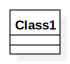
\includegraphics{language/main}
\caption{This is the caption of the figure displaying a white eagle and
a white horse on a snow field}
\end{figure}

\section{The Extensible Compiler}\label{sec:compiler}
%
\section{The Development Workflow}\label{sec:workflow}
%
\section{The Cost-Benefit Analysis Model}\label{sec:cba}
%
\section{Conclusion}\label{sec:conclusion}

The CML language and compiler make it possible to specify,
in a single high-level language,
the concepts of ever-changing, increasingly distributed software systems.

As opposed to implementing these concepts, their properties and associations in each target language,
from a single CML model,
the CML extensible templates generate code that
keeps the implementations 
(across the different platforms and technologies) 
consistent with the specification.
Also, as the technology landscape evolves,
these textual CML models can be reused to generate code in new target languages and technologies.

The initial version of CML has been designed to validate this textual, model-driven approach of development.
Practical application of CML in software development is needed in order to provide qualitative evidence that
CML can indeed be used as a single source to implement multiple targets.
Quantitative cost-benefit analysis
(based on the implementation effort of hand-written vs generated lines-of-code, perhaps using a method adapted from the work of Gaffney et al \cite{gaffney})
may also provide data
that shows whether the investment -- made on the development of CML models -- pays off. The data collected, together with the feedback provided by software developers, should then inform the iterative design of new CML features.

\appendix
\section{The Language Specification}\label{sec:spec}
%
This appendix provides a formal description of the concrete syntax, along with its mapping to the abstract syntax.

\subsection{Notation}

The notation is based on BNF, but it also specifies the construction of the AST. Each grammar production that must be instantiated into a AST node is followed by a block specifying the node properties. The property may be assigned by a constant, by a terminal token, or by a reference to other nodes. Super-nodes may reference the sub-nodes (attribute synthesis in attributed grammars.) The sub-nodes may also reference super-nodes (attribute inheritance in attributed grammars.) 

\subsection{Extended Grammar}

TODO: Update the grammar before submitting the article.

\verbatimfont{\tiny}
\begin{verbatim}
root Module: (Concept | Target)*
{
    elements = Concept* + Target*;
}

node Concept: 'abstract'? 'concept' NAME (':' AncestorList)? (';' | PropertyList)
{
    name = NAME;
    abstract = 'abstract'?;

    properties = Property*;
    properties.typeRequired = false;
    properties.typeAllowed = true;

    ancestors = for name in AncestorList.NAME* | map Model.concept[name];
    missingAncestors = AncestorList.NAME* - ancestors.name;
}

node Target: 'target' NAME PropertyList
{
    name = NAME;

    properties = Property*;
    properties.typeRequired = false;
    properties.typeAllowed = false;
}

node PropertyList: '{' (Property ';')* '}';

node Property: NAME (':' Type)? ('=' STRING)?
{
    name = NAME;
    value = unwrap(STRING?);
    type = Type?;
}

node ancestorListNode: NAME (',' NAME)*;

node Type: NAME CARDINALITY?
{
    name = NAME;
    cardinality = CARDINALITY?;
}

token NAME: ('A'..'Z' | 'a'..'z') ( 'A'..'Z' | 'a'..'z' | '0'..'9' | '_' )*;
token STRING: '"' .*? '"';
token CARDINALITY: ('?' | '*');

function unwrap(str: String): String
{
    let /"?(<value>.*?)"?/ = str;

    return value or else str;
}
\end{verbatim}

%
\bibliographystyle{spmpsci}
\bibliography{references}
%
\end{document}
